\section{}
In questa sezione si commenta il cambiamento del guadagno ottenuto inserendo la resistenza $R_{res}=\SI{96.1\pm 1.1}{\ohm}$  in parallelo alla resistenza di emettitore, disaccoppiata in continua con un condensatore da $C_E=\SI{100}{\micro\farad} (10\%)$. Teoricamente questa modifica è molto interessante in quanto permette, per piccoli segnali, di lavorare intorno al vecchio punto di lavoro, ma di spostarsi su una retta di carico diversa. Dati e fit sono mostrati in figura \ref{f:VinVout2}. La procedure di analisi e presa dati sono state essenzialmente identiche a quelle attuate per il punto 2, ma, avendo avuto cura di limitarsi a piccoli segnali di ingresso in presa dati, non c'è stato bisogno di tagliare i dati.
% A: il valore della resistenza me lo sono inventato, non si trova in nessun file!!!!!!
% V: CRISTO. l'ho inventato meglio...
\begin{figure}
\centering
	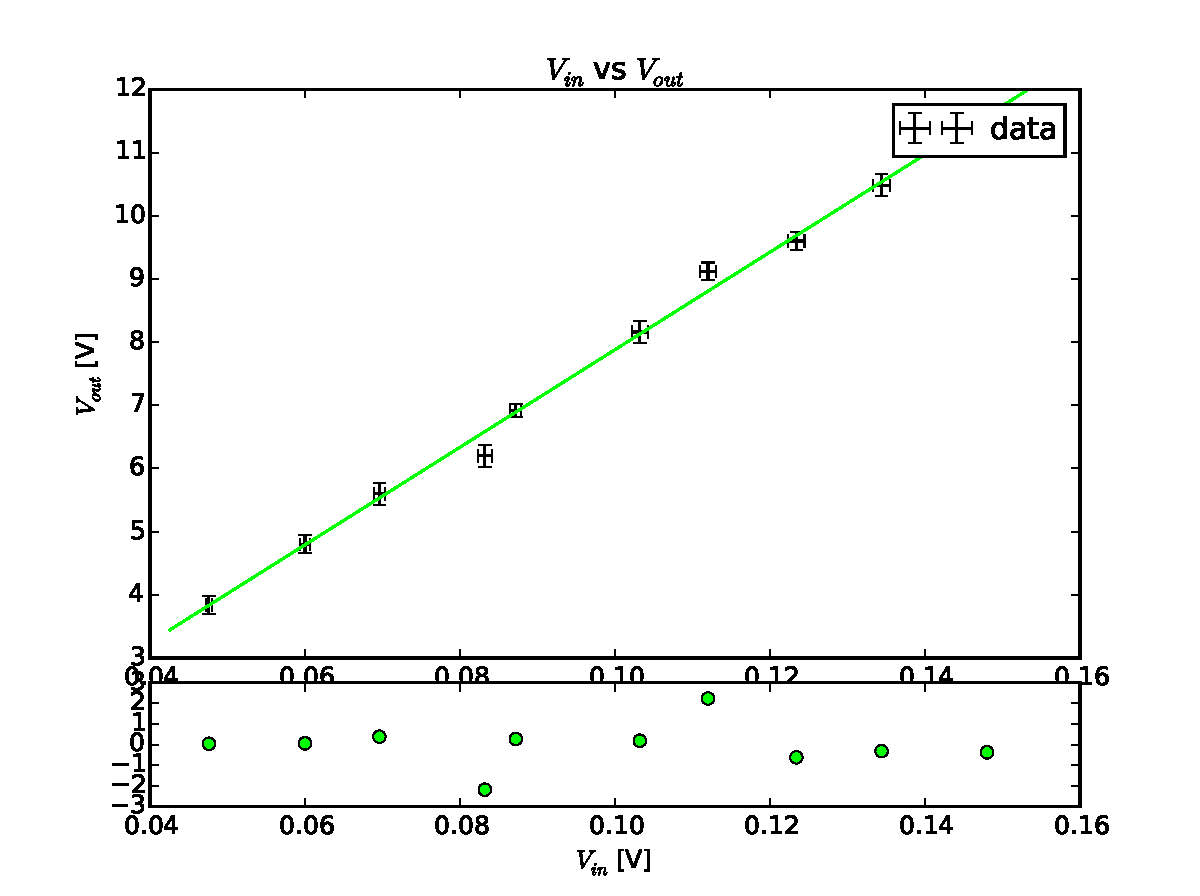
\includegraphics[scale=0.8]{VinVout2.pdf}
	\caption{Andamento lineare, fittato con un cutoff di $\SI{1.5}{\V}$.\label{f:VinVout2}}
\end{figure}

Si sono ottenuti dunque i seguenti parametri di fit:\\
$\alpha=77.2 \pm 1.7$\\
$\beta=\SI{0.16 \pm 0.17}{\V}$\\
$corr_{\alpha, \beta}=-0.94$\\
$\chi^2= 10.68$ ($8$ DoF, $p_{\chi^2>10.68} = 0.21)$\\

Si può notare che $\alpha$ non è neanche lontanamente compatibile con $R_c/R_{res}\approx 100$ entro l'errore. Questo è però un fenomeno atteso. Infatti non si può più pensare che $h_{ie}<<h_{fe}(R_e \paral R_{res})$. Si può utilizzare il valore di $h_{ie}$ misurato durante la scorsa esperienza ($178 \pm 10$) per stimare $h_{ie}=R_c*h_{fe}/\alpha-(h_{fe}+1)( R_e \paral R_{res} )=\SI{6.8\pm 0.6}{\kohm}$\footnote{Per il calcolo dell'errore si è assunto che le misure delle resistenze, fatte con lo stesso strumento, avessero errore, dato da manuale, scorrelato. Questo potrebbe non essere del tutto vero, dunque l'errore potrebbe essere minore.}. Il valore $h_{ie}$ di riferimento non è riportato dal datasheet, ma i valori tipici dovrebbero essere dell'ordine di grandezza del \si{\kohm}.

%Inserendo questo valore di $h_{ie}$ nel calcolo del guadagno si ottiene, tralasciando i condensatori, $A_V = \SI{74(5)}{}$, in accordo con quanto osservato.
%Questo è ovvio essendo stato trovato invertendo la formula del guadagno!!!
%oh derp, pensavo fosse stato fatto con il guadagno in continua